\subsection{Đề 05}
\Opensolutionfile{ans}[ans/ans-2-B1-De1-LC]
\caulc
\begin{ex}%[Câu 1]%[1D1N4-5]
	Cho tập hợp $C=\left\lbrace x \in \mathbb{R} | -4 \leq x \leq 0 \right\rbrace$. Tập hợp $C$ được viết dưới dạng tập hợp nào sau đây?
	\choice
	{$C=(-4;0]$}
	{$C=(-4;0)$}
	{$C=[-4;0)$}
	{\True $[-4;0]$}
	\loigiai{
	Ta có $C=[-4;0]$.
	}
\end{ex}

\begin{ex}%[Câu 2]%[1D1N1-2]
	Cho hàm số $y=f(x)$ có đồ thị như hình bên dưới
	\begin{center}
		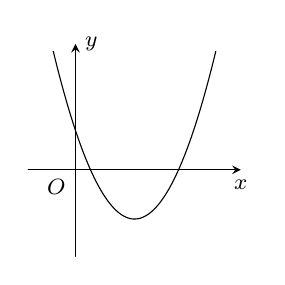
\begin{tikzpicture}[scale=0.5, font=\footnotesize, line join=round, line cap=round, >=stealth]
			\def\xmin{-1}\def\xmax{4}\def\ymin{-2}\def\ymax{3}
			\draw[->] (\xmin-0.2,0)--(\xmax+0.2,0) node[below] {\footnotesize $x$};
			\draw[->] (0,\ymin-0.2)--(0,\ymax+0.2) node[right] {\footnotesize $y$};
			\draw (0,0) node [below left] {\footnotesize $O$};
			\foreach \x in {}\draw (\x,0.1)--(\x,-0.1) node [below] {\footnotesize $\x$};
			\foreach \y in {}\draw (0.1,\y)--(-0.1,\y) node [left] {\footnotesize $\y$};
			\clip (\xmin,\ymin) rectangle (\xmax,\ymax);
			\draw[smooth,samples=200,domain=\xmin:\xmax] plot (\x,{1*((\x)^2)+-3*\x+1});
		\end{tikzpicture}
	\end{center}
	Biết $y=f(x)$ là một trong các hàm số dưới đây
	\choice
	{$y=2x+1$}
	{$y=x^2-3x-1$}
	{\True $y=x^2-3x+1$}
	{$y=x^2+1$}
	\loigiai{
		Từ hình vẽ ta thấy được đồ thị hàm số $y=f(x)$ là một parabol nên A sai.\\
		Có $f(0)>0$ nên phương án B sai.\\
		Có hoành độ đỉnh dương nên D sai.
	}
\end{ex}

\begin{ex}%[Câu 3]%[1D1N3-2]
	Cho tam giác $ABC$ có $AB=7$cm, $AC=5$cm, $\widehat{(C)}=60^\circ$. Độ dài cạnh $BC$ bằng với giá trị nào sau đây
		\choice 
		{$6{,}25$cm}
		{$3$cm}
		{$6{,}24$cm}
		{\True $8$cm}
	\loigiai{
		Ta có $AB^2=CB^2+CA^2-2CB \cdot CA \cdot \cos \widehat{(C)} \Leftrightarrow CB^2-5CB-24=0 \Leftrightarrow \hoac{&CB=8 \text{ (Nhận)}\\&CB=-3 \text{ (Loại)}.}$
	}
\end{ex}

\begin{ex}%[Câu 4]%[1D1H1-1]
	Trên đường thẳng $MN$ lấy điểm $P$ sao cho $\vec{MN}=-3\vec{MP}$. Điểm $P$ được xác định đúng trong hình vẽ nào sau đây?\\
	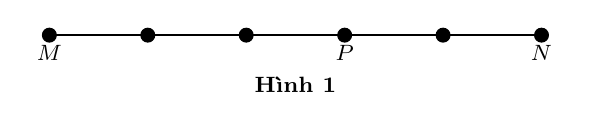
\begin{tikzpicture}[scale=1.25, font=\footnotesize, line join=round, line cap=round, >=stealth]
		\draw[thick] (0,0) -- (5,0);
		\filldraw (1,0) circle (2pt);
		\filldraw (2,0) circle (2pt);
		\filldraw (4,0) circle (2pt);
		\filldraw (0,0) circle (2pt) node[below] {$M$};
		\filldraw (3,0) circle (2pt) node[below] {$P$};
		\filldraw (5,0) circle (2pt) node[below] {$N$};
		\node at (2.5,-0.5) {\textbf{Hình 1}};
	\end{tikzpicture}
	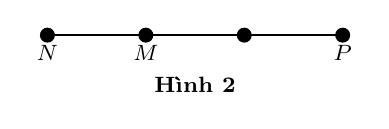
\begin{tikzpicture}[scale=1.25, font=\footnotesize, line join=round, line cap=round, >=stealth]
		\draw[thick] (0,0) -- (3,0);
		\filldraw (2,0) circle (2pt);
		\filldraw (0,0) circle (2pt) node[below] {$N$};
		\filldraw (1,0) circle (2pt) node[below] {$M$};
		\filldraw (3,0) circle (2pt) node[below] {$P$};
		\node at (1.5,-0.5) {\textbf{Hình 2}};
	\end{tikzpicture}\\
	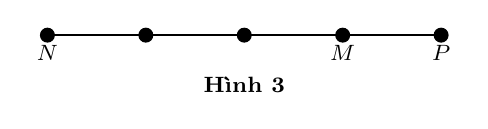
\begin{tikzpicture}[scale=1.25, font=\footnotesize, line join=round, line cap=round, >=stealth]
		\draw[thick] (0,0) -- (4,0);
		\filldraw (1,0) circle (2pt);
		\filldraw (2,0) circle (2pt);
		\filldraw (0,0) circle (2pt) node[below] {$N$};
		\filldraw (3,0) circle (2pt) node[below] {$M$};
		\filldraw (4,0) circle (2pt) node[below] {$P$};
		\node at (2,-0.5) {\textbf{Hình 3}};
	\end{tikzpicture}
	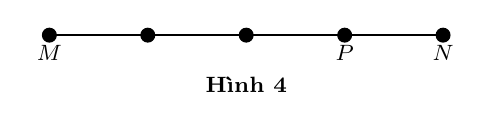
\begin{tikzpicture}[scale=1.25, font=\footnotesize, line join=round, line cap=round, >=stealth]
		\draw[thick] (0,0) -- (4,0);
		\filldraw (1,0) circle (2pt);
		\filldraw (2,0) circle (2pt);
		\filldraw (0,0) circle (2pt) node[below] {$M$};
		\filldraw (4,0) circle (2pt) node[below] {$N$};
		\filldraw (3,0) circle (2pt) node[below] {$P$};
		\node at (2,-0.5) {\textbf{Hình 4}};
	\end{tikzpicture}
	\choice
	{\True Hình 3}
	{Hình 2}
	{Hình 4}
	{Hình 1}
	\loigiai{
		Vì $\vec{MN}=-3\vec{MP} \Leftrightarrow \vec{MN}=3\vec{PM}$\\
		Vậy vectơ $\vec{MN}$ cùng phương và gấp 3 lần so với vectơ $\vec{PM} \Rightarrow$ Hình 3 thỏa mãn.
	}
\end{ex}

\begin{ex}%[Câu 5]%[1D2H3-1]
	Cặp số nào sau đây là nghiệm của hệ bất phương trình $\heva{&x-2y \le 8\\&3x+y>3}$?
	\choice
	{$(0;1)$}
	{$(0;-4)$}
	{$(1;-1)$}
	{\True $(1;1)$}
	\loigiai{ 
		Lần lượt thay các bộ số ở các phương án vào hệ bất phương trình ta được một nghiệm của hệ bất phương trình trên là $(1;1)$.
	}
\end{ex}

\begin{ex}%[Câu 6]%[1D2H1-5]
	Cho hình bình hành $ABCD$ có tâm $O$. Khẳng định nào sau đây đúng
	\choice
	{\True $\vec{AB}-\vec{AC}=\vec{DA}$}
	{$\vec{AO}-\vec{AC}=\vec{BO}$}
	{$\vec{AO}-\vec{BO}=\vec{CD}$}
	{$\vec{AO}-\vec{BO}=\vec{BD}$}
	\loigiai{
		Ta có $\vec{AB}-\vec{AC}=\vec{CB}$. Do $ABCD$ là hình bình hành nên $\vec{CB}=\vec{DA} \Rightarrow \vec{AB}-\vec{AC}=\vec{DA}$.
	}
\end{ex}

\begin{ex}%[Câu 7]%[1D5N1-2]
	Cho $\vec{a}$ và $\vec{b}$ là hai vectơ cùng hướng và đều khác $\vec{0}$. Mệnh đề nào sau đây đúng?
	\choice
	{\True $\vec{a} \cdot \vec{b}=\left|\vec{a}\right|\cdot\left|\vec{b}\right|$}
	{$\vec{a}\cdot\vec{b}=0$}
	{$\vec{a}\cdot\vec{b}=-1$}
	{$\vec{a} \cdot \vec{b}=-\left|\vec{a}\right|\cdot\left|\vec{b}\right|$}
	\loigiai{
	Ta có $\vec{a} \cdot \vec{b}=\left|\vec{a}\right|\cdot\left|\vec{b}\right|\cdot \cos\left(\vec{a},\vec{b}\right)$.\\
	Do $\vec{a}$ và $\vec{b}$ là hai vectơ cùng hướng nên $\left(\vec{a}, \vec{b}\right)=0^\circ \Rightarrow \cos\left(\vec{a},\vec{b}\right)=1$.\\
	Vậy $\vec{a} \cdot \vec{b}=\left|\vec{a}\right|\cdot\left|\vec{b}\right|$.
	}
\end{ex}

\begin{ex}%[Câu 8]%[1D3H2-3]
		Số tiền quỹ lớp $10A$ còn lại là $a=1\,647\,500$ (đồng) với độ chính xác $d=500$ (đồng). Hãy viết số quy tròn của số $a$?
		\choice
		{\True Số quy tròn của $a$ là $1\,648\,000$ (đồng)}
		{Số quy tròn của $a$ là $1\,647\,000$ (đồng)}
		{Số quy tròn của $a$ là $1\,649\,000$ (đồng)}
		{Số quy tròn của $a$ là $1\,650\,000$ (đồng)}
	\loigiai{
		Vì độ chính xác $d=500$ đến hàng trăm nên ta quy tròn số gần đúng $a$ đến hàng nghìn.\\
		Vậy số quy tròn của $a$ là $1\,648\,000$ (đồng).
	}
\end{ex}

\begin{ex}%[Câu 9]%[1H4V2-2]
	Cho mẫu thống kê số lượng trứng gà thu hoạch được trong ngày của các trại $\{28;16;13;18;12;28;13;19\}$. Trung vị của mẫu số liệu trên là bao nhiêu?
	\choice
	{$14$}
	{\True $17$}
	{$18$}
	{$20$}
	\loigiai{
		Mẫu thống kê có 8 số liệu được sắp xếp theo thứ tự không giảm là:\\
		$12;13;13;16;18;19;28;28$, nên trung vị của mẫu số liệu trên là $M_{\mathrm{e}}=\dfrac{16+18}{2}=17$.
	}
\end{ex}

\begin{ex}%[Câu 10]%[1D5H2-3]
	Tiền thưởng (đơn vị: triệu đồng) của cán bộ và nhân viên trong công ty $A$ được cho ở bảng dưới đây:
	\begin{center}
		\begin{tabular}{|c|c|c|c|c|c|c|}
		\hline
		Tiền thưởng & $12$ & $13$ & $14$ & $15$ & $16$ & Tổng \\ \hline
		Tần số      & $25$ & $15$ & $11$ & $16$ & $17$ & $84$ \\ \hline
	\end{tabular}
	\end{center}
	Tính mốt $M_\text{o}$.
	\choice
	{$M_\text{o}=15$}
	{\True $M_\text{o}=12$}
	{$M_\text{o}=10$}
	{$M_\text{o}=16$}
	\loigiai{
		Trong mẫu số liệu mốt là giá trị xuất hiện nhiều nhất.\\
		Vậy $M_\text{o}=12$
	}
\end{ex}

\begin{ex}%[Câu 11]%[1D1H2-2]
	Sau khi tổng kết cuối tháng quản lý của một quán trà sữa tổng kết lại lợi nhuận (đơn vị: \$) trong 20 ngày qua là:\\
	$4;5;6;8;9;11;13;16;16;18;20;21;25;30;31;33;36;37;40;41$.\\
	Khoảng tứ phân vị của mẫu số liệu trên là:
	\choice
	{$20$}
	{\True $22$}
	{$24$}
	{$26$}
	\loigiai{
		Số liệu trên đã sắp xếp theo thứ tự không giảm.\\
		Ta có $Q_1=10$; $Q_2=19$; $Q_3=32$.\\
		Vậy khoảng tứ phân vị của mẫu số liệu trên là $\Delta_Q=Q_3-Q_1=22$.
	}
\end{ex}

\begin{ex}%[Câu 12]%[1D2H2-7]
	Cho tam giác đều $ABC$ có trọng tâm $G$ và độ dài cạnh bằng $a$. Tính tích vô hướng $\vec{AB} \cdot \vec{AG}$
	\choice
	{$\dfrac{a^2\sqrt{3}}{6}$}
	{$\dfrac{3a^2}{4}$}
	{$\dfrac{a^2\sqrt{3}}{4}$}
	{\True $\dfrac{a^2}{2}$}
	\loigiai{
		\begin{center}
			\begin{tikzpicture}[scale=1, font=\footnotesize, line join=round, line cap=round, >=stealth]
			\coordinate (C) at (-2,0);
			\coordinate (B) at (0,0);
			\coordinate (A) at (-1,{sqrt(3)}) ;
			\coordinate (H) at ($(B)!0.5!(C)$);
			\coordinate (G) at ($ (A)!2/3!(H) $) ;
			\draw (A)--(B)--(C)--cycle;
			\draw (A)--(H);
			\filldraw (A) circle (1.5pt) node[above]{$A$};
			\filldraw (B) circle (1.5pt)  node[below]{$B$};
			\filldraw (C) circle (1.5pt)  node[below]{$C$};
			\filldraw (G) circle (1.5pt)  node[below left]{$G$};
			\filldraw (H) circle (1.5pt) node[below]{$H$};
		\end{tikzpicture}
		\end{center}
		Ta có $\heva{&\vec{AB} \cdot \vec{AG}=\left|\vec{AB}\right| \cdot \left|\vec{AG}\right| \cdot \cos\left(\vec{AB},\vec{AG}\right)\\&\left|\vec{AB}\right|=AB=a\\&\left|\vec{AG}\right|=AG=\dfrac{2}{3}AH=\dfrac{a\sqrt{3}}{3}\\&\left(\vec{AB},\vec{AG}\right)=60^\circ.}$\\
		Vậy $\vec{AB} \cdot \vec{AG}=a \cdot \dfrac{a\sqrt{3}}{3} \cdot \cos 30^\circ=\dfrac{a^2}{2}$.
	}
\end{ex}
\Closesolutionfile{ans}
\indapan{6}{ans/ans-2-B1-De1-LC}
%-------------------------------------------
\Opensolutionfile{ans}[ans/ans-2-B1-De1-DS]
\cauds
\begin{ex}%[Câu 1]%[1D5V2-3]
	Cho hàm số $y=-x^2-2$. Khi đó
	\choiceTF
	{\True Đồ thị của hàm số có đỉnh $I(0;-2)$}
	{Đồ thị của hàm số có trục đối xứng là đường thẳng $x=1$}
	{\True Đồ thị của hàm số giao điểm với trục $Oy$ là $I(0;-2)$}
	{\True $\forall x \in \mathbb{R}$ thì $y<0$}
	\loigiai{
		Tập xác định $\mathscr{D}=\mathbb{R}$, đỉnh $I(0;-2)$, trục đối xứng là đường thẳng $x=0$.\\
		Xét $y=-x^2-2 \Rightarrow y<-2$ vì $-x^2 \leq 0$.
	}
\end{ex}

\begin{ex}%[Câu 2]%[1H4H4-6]
	Cho hình ngũ giác $ABCDE$. Xét các vectơ có điểm đầu và điểm cuối là các đỉnh của đa giác.
	\choiceTF
	{Có $10$ vectơ (khác $\vec{0}$) được lập ra từ các cạnh của ngũ giác}
	{Có $5$ vectơ (khác $\vec{0}$) được lập ra từ các đường chéo của ngũ giác}
	{Có $3$ vectơ (khác $\vec{0}$) được lập ra từ các cạnh của tam giác $ABC$}
	{Có $4$ vectơ (khác $\vec{0}$) được lập ra từ các đường chéo của tứ giác $ABCD$}
	\loigiai{
		\begin{itemchoice}
			\itemch Đúng. Vì ngũ giác có $5$ cạnh do đó có $10$ vectơ tạo thành từ các cạnh.
			\itemch Sai. Vì ngũ giác có $5$ đường chéo do đó có $10$ vectơ tạo thành từ các đường chéo.
			\itemch Đúng. Vì có $6$ vectơ (khác $\vec{0}$) được lập ra từ các cạnh của tam giác $ABC$.
			\itemch Sai. Vì có $4$ vectơ (khác $\vec{0}$) được lập ra từ các đường chéo của tứ giác $ABCD$.
		\end{itemchoice}
	}
\end{ex}

\begin{ex}%[Câu 3]%[1D2V1-1]
	Cho hình bình hành $ABCD$. Gọi $I,J$ lần lượt là trung điểm $BC$ và $CD$. Khi đó
	\choiceTF
	{\True $\vec{AC}=\vec{AB}+\vec{AD}$}
	{$\vec{AI}=\vec{AC}+\vec{AB}$}
	{$\vec{AI}=\vec{AB}+\dfrac{3}{2}\vec{AD}$}
	{$\vec{AJ}=\dfrac{1}{2}\vec{AB}+\dfrac{1}{2}\vec{AD}$}
	\loigiai{
		\begin{center}
			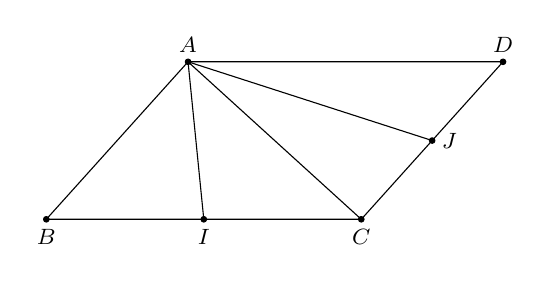
\begin{tikzpicture}[scale=1, font=\footnotesize, line join=round, line cap=round, >=stealth]
		\coordinate (A) at (1.8,2);
		\coordinate (B) at (0,0);
		\coordinate (C) at (4,0);
		\coordinate (D) at (5.8,2);
		\coordinate (I) at (2,0);
		\coordinate (J) at (4.9,1);
		\draw (A)--(B)--(C)--(D)--(A);
		\draw (A)--(I);
		\draw (A)--(J);
		\draw (A)--(C);
		\filldraw (A) circle(1pt) node[above]{$A$};
		\filldraw (B) circle(1pt) node[below]{$B$};
		\filldraw (C) circle(1pt) node[below]{$C$};
		\filldraw (D) circle(1pt) node[above]{$D$};
		\filldraw (J) circle(1pt) node[right]{$J$};
		\filldraw (I) circle(1pt) node[below]{$I$};
		\end{tikzpicture}
		\end{center}
		\begin{itemchoice}
		\itemch Đúng.
		\itemch Sai. Vì $\vec{AI}=\dfrac{1}{2}\vec{AC}+\dfrac{1}{2}\vec{AB}$.
		\itemch Sai. Vì $\vec{AI}=\dfrac{1}{2}\left(\vec{AB}+\vec{AD}\right)+\dfrac{1}{2}\vec{AB}$.
		\itemch Sai. Vì $\vec{AJ}=\dfrac{1}{2}\left(\vec{AD}+\vec{AC}\right)=\dfrac{1}{2}\vec{AD}+\dfrac{1}{2}\left(\vec{AB}+\vec{AD}\right)=\dfrac{1}{2}\vec{AB}+\vec{AD}$.
		\end{itemchoice}
	}
\end{ex}

\begin{ex}%[Câu 4]%[1D1V5-3]
	Mẫu số liệu dưới đây thống kê thời gian chờ xe buýt (đơn vị: phút) của $10$ học sinh ở cùng một bến.
	$$1;4;5;6;6;8;10;11;12;25$$
	\choiceTF
	{\True Số trung bình cộng của mẫu số liệu là $\overline{x}=8{,}8$ (phút)}
	{Khoảng tứ phân vị của mẫu số liệu là $\Delta_Q=5$ (phút)}
	{Độ lệch chuẩn của mẫu số liệu là $s \approx 5{,}27$ (phút)}
	{\True $25$ là giá trị bất thường của mẫu số liệu}
	\loigiai{
		\begin{itemchoice}
			\itemch Đúng. Vì $\overline{x}=\dfrac{1+4+5+6+6+8+10+11+12+25}{10}=8{,}8$ (phút).
			\itemch Đúng. Trung vị của mẫu số liệu là $\dfrac{6+8}{2}=7$ (phút).\\
			Trung vị của dãy $1;4;5;6;6$ là $5$. Trung vị của dãy $8;10;11;12;25$ là $11$.\\
			Vậy tứ phân vị của mẫu số liệu là $Q_1=5$ (phút), $Q_2=7$ (phút), $Q_3=11$ (phút).\\
			Khoảng biến thiên của mẫu số liệu là $R=25-1=24$ (phút).\\
			Khoảng tứ phân vị của mẫu số liệu là $\Delta_Q=11-5=6$ (phút).
			\itemch Sai. Ta có $(1-8{,}8)^2+(4-8{,}8)^2+(5-8{,}8)^2+(6-8{,}8)^2\cdot2+(8-8{,8})^2+(10-8{,}8)^2+(11-8{,}8)^2+(12-8{,}8)^2+(25-8{,}8)^2=393{,}6$.\\
			Suy ra phương sai của mẫu số liệu là $s^2=\dfrac{393{,6}}{10}=39{,}36$.\\
			Độ lệch chuẩn của mẫu số liệu là $s=\sqrt{39{,}36}\approx6{,}27$ (phút).
			\itemch Đúng. Ta có $Q_1-\dfrac{3}{2}\Delta_Q=5-\dfrac{3}{2}\cdot6=-4$, $Q_3+\dfrac{3}{2}\cdot\Delta_Q=11+\dfrac{3}{2}=20$. Vì $25>20$ nên $25$ là giá trị bất thường của mẫu số liệu.
		\end{itemchoice}
	}
\end{ex}
\Closesolutionfile{ans}
\indapan{3}{ans/ans-2-B1-De1-DS}
%-------------------------------------------
\Opensolutionfile{ans}[ans/ans-2-B1-De1-KQ]
\caukq
\begin{ex}%[Câu 1]%[1D1H2-3]
	Một người nông dân thả $1\,000$ con cá giống vào hồ nuôi vừa mới đào. Biết rằng sau mỗi năm thì số lượng cá trong hồ tăng thêm $x$ lần số lượng cá ban đầu và $x$ không đổi. Bằng cách thay đổi kĩ thuật nuôi và thức ăn cho cá. Hỏi sau hai năm để số cá trong hồ là $9000$ con thì tốc độ tăng trưởng cá trong hồ là bao nhiêu? Biết tốc độ tăng mỗi năm là không đổi
	\shortans[0]{$5$}
	\loigiai{
		Sau một năm số lượng các trong hồ là $1\,000+1\,000x=1\,000(1+x)$ (con).\\
		Sau hai năm số lượng cá trong hồ là $1\,000(1+x)+1\,000(1+x)x=1\,000(1+x)^2$ (con).\\
		Điều kiện $x>0$. Để số lượng cá trong hồ sau hai năm là $9000$ thì ta có:\\
		$\Rightarrow 1\,000(1+x)^2=9\,000 \Leftrightarrow (1+x)^2=9 \Leftrightarrow \hoac{&x=5\text{ (nhận)}\\&x=-7\text{ (loại)}.}$\\
		Vậy tốc độ tăng thêm số lượng cá trong hồ sau mỗi năm là $5$ lần số lượng cá ban đầu.
	}
\end{ex}

\begin{ex}%[Câu 2]%[1D2V2-7]
	Hai chiếc tàu thủy cùng xuất phát từ vị trí $A$, đi thẳng theo hai hướng tạo với nhau một góc $60^\circ$. Tàu thứ nhất chạy với tốc độ $20$ km/h, tàu thứ hai chạy với tốc độ $30$ km/h. Hỏi sau $3$ giờ hai tàu cách nhau bao nhiêu km?
	\shortans[0]{$60{,}5$}
	\loigiai{
		Ta có quãng đường tàu thứ nhất đi được là $s_1=v_1t=20\cdot3=60$ (km).\\
		Quãng đường tàu thứ hai đi được là $s_2=v_2t=30\cdot3=90$ (km).\\
		Tam giác $ABC$ với $B$ là vị trí tàu thứ nhất chạy đến sau $3$ giờ, nghĩa là $AB=s_1=60$ km; $C$ là vị trí tàu thứ hai chạy đến sau $3$ giờ, nghĩa là $AC=s_2=90$ km.\\
		$$BC^2=AB^2+AC^2-2AB\cdot AC \cos \widehat{BAC}\Leftrightarrow BC^2=60^2+90^2-2\cdot60\cdot90\cdot \cos 60^\circ \Leftrightarrow BC^2=6300$$\\
		Vậy khoảng cách hai tàu sau $3$ giờ chạy là $BC=30\sqrt{7}$.
	}
\end{ex}

\begin{ex}%[Câu 3]%[1D2V3-8]
	Cho tứ giác $ABCD$. Gọi $M$, $N$, $P$, $Q$ lần lượt là trung điểm của $AB$, $BC$, $CD$, $DA$. Từ các điểm đã cho tìm các vectơ cùng hướng với vectơ $\vec{MN}$.
	\shortans[0]{$2$}
	\loigiai{
		Ta có $MN,PQ$ lần lượt là đường trung bình của tam giác $ABC$ và $ADC$.\\
		Vậy $MN\parallel PQ, MN=PQ$ (do cùng song song và bằng một nửa $AC$). Do đó $MNPQ$ là hình bình hành.\\
		Vậy các vectơ cùng hướng với vectơ $\vec{MN}$ là $\vec{PQ},\vec{AC}$.
	}
\end{ex}

\begin{ex}%[Câu 4]%[1D5H1-4]
	Cho ba lực $\vec{F_1}=\vec{MA}$, $\vec{F_2}=\vec{MB}$, $\vec{F_3}=\vec{MC}$ cùng tác động vào một vật tại điểm $M$ và vật đứng yên. Cho biết cường độ của $\vec{F_1}$, $\vec{F_2}$ đều bằng $100$N và góc $\widehat{AMB}=90^\circ$. Khi đó tính cường độ của lực $\vec{F_3}$ (làm tròn đến hàng đơn vị).
	\begin{center}
		\begin{tikzpicture}[scale=1, font=\footnotesize, line join=round, line cap=round, >=stealth]
			\coordinate (C) at (-3,0);
			\coordinate (B) at (2,-2);
			\coordinate (A) at (2,2);
			\coordinate (M) at (0,0);
			\draw[->,thick] (M)--(C);
			\draw[->,thick] (M)--(A);
			\draw[->,thick] (M)--(B);
			\filldraw (A) circle(1.5pt) node[above]{A};
			\filldraw (M) circle(1.5pt) node[right]{M};
			\filldraw (B) circle(1.5pt) node[below]{B};
			\filldraw (C) circle(1.5pt) node[above]{C};
			\node[above] at ($(C)!0.5!(M)$){$\vec{F_3}$};
			\node[right] at ($(A)!0.5!(M)$){$\vec{F_1}$};
			\node[right] at ($(B)!0.5!(M)$){$\vec{F_2}$};
		\end{tikzpicture}
	\end{center}
	\shortans[0]{$141$}
	\loigiai{
		Vẽ hình vuông $ADBM$, cạnh $MA=100$ thì $MD=100\sqrt{2}$. Theo qui tắc hình bình hành có $\vec{MA}+\vec{MB}=\vec{MD}$. Vật đứng yên khi $\vec{F_3}=-\vec{MD}$. Suy ra cường độ của lực $\vec{F_3}$ là $\left|\vec{F_3}\right|=100\sqrt{2}$.
		\begin{center}
			\begin{tikzpicture}[scale=1, font=\footnotesize, line join=round, line cap=round, >=stealth]
				\coordinate (C) at (-3,0);
				\coordinate (B) at (2,-2);
				\coordinate (A) at (2,2);
				\coordinate (M) at (0,0);
				\coordinate (D) at (4,0);
				\draw[->,thick] (M)--(C);
				\draw[->,thick] (M)--(A);
				\draw[->,thick] (M)--(B);
				\draw[dashed] (A)--(D);
				\draw[dashed] (M)--(D);
				\draw[dashed] (B)--(D);
				\filldraw (A) circle(1.5pt) node[above]{$A$};
				\filldraw (M) circle(1.5pt) node[below left]{$M$};
				\filldraw (B) circle(1.5pt) node[below]{$B$};
				\filldraw (C) circle(1.5pt) node[above]{$C$};
				\filldraw (D) circle(1.5pt) node[right]{$D$};
				\node[above] at ($(C)!0.5!(M)$){$\vec{F_3}$};
				\node[right] at ($(A)!0.5!(M)$){$\vec{F_1}$};
				\node[right] at ($(B)!0.5!(M)$){$\vec{F_2}$};
			\end{tikzpicture}
		\end{center}
	}
\end{ex}

\begin{ex}%[Câu 5]%[1D3H3-3]
	Bảng sau thống kê số lớp và số học sinh theo từng khối ở một trường trung học phổ thông.
	\begin{center}
		\begin{tabular}{|c|c|c|c|}
		\hline
		Khối 		& $10$ & $11$ & $12$\\
		\hline
		Số lớp		& $14$ & $13$ & $15$\\
		\hline
		Số học sinh & $555$ & $519$ & $615$\\
		\hline
	\end{tabular}
	\end{center}
	Hiệu trưởng trường đó cho biết sĩ số mỗi lớp trong tường đều không vượt quá $40$ học sinh. Có bao nhiêu khối lớp bị thống kê sai?
	\shortans[0]{$1$}
	\loigiai{
		Số lượng học sinh khối $10$ thực tế là $40\cdot14=560>555$. Vậy thống kê học sinh lớp $10$ đúng.\\
		Số lượng học sinh khối $11$ thực tế là $40\cdot13=520>519$. Vậy thống kê học sinh lớp $11$ đúng.\\
		Số lượng học sinh khối $12$ thực tế là $40\cdot15=600>615$. Vậy thống kê học sinh lớp $12$ sai.
	}
\end{ex}

\begin{ex}%[Câu 6]%[1D1C4-6]
	Bảng số liệu sau thống kê nhiệt độ tại Thành phố Hồ Chí Minh trong một lần đo vào một ngày của năm 2021 
	\begin{center}
		\begin{tabular}{|c|c|c|c|c|c|c|c|c|}
	\hline
	Giờ đo			& $1$h & $4$h & $7$h & $10$h & $13$h & $16$h & $19$h & $22$h \\
	\hline
	Nhiệt độ (độ C)	& $27$ & $26$ & $28$ & $32$ & $34$ & $35$ & $30$ & $28$ \\
	\hline
	\end{tabular}
	\end{center}
	Tìm độ lệch chuẩn của mẫu số liệu đã cho (làm tròn kết quả đến hàng phần trăm).
	\shortans[0]{$3{,}12$}
	\loigiai{
		Số trung bình là $\overline{x}=\dfrac{27+26+\ldots+30+28}{8}=30$.\\
		Phương sai $s^2=\dfrac{1}{8}\left[(x_1-\overline{x})^2+(x_2-\overline{x})^2+\ldots+(x_8-\overline{x})^2\right]$\\$s^2=\dfrac{1}{8}\left[(27-30)^2+(26-30)^2+\ldots+(28-30)^2\right]=9{,}75$.\\
		Độ lệch chuẩn $s=\sqrt{s^2}\approx3{,}12$.
	}
\end{ex}
\Closesolutionfile{ans}
\indapan{6}{ans/ans-2-B1-De1-KQ}